\chapter{Les Nombres Relatifs}


\section{Introduction}

Nous avons vu que nous pouvons créer des nombres de plus en plus grands. Pour le montrer, faisons une démonstration rapide. Supposons qu'il existe un nombre qui soit le plus grand nombre possible. Prenons ensuite ce nombre plus 1. Nous savons que ce nouveau nombre est plus grand que le nombre qui était supposé être le plus grand possible, ce qui ne fait pas de sens. On peux toujours créer des nombres de plus en plus grand. Cependant, nous ne pouvons pas faire l'inverse. Nous ne connaissons (pour l'instant du moins) aucun nombre plus petit que 0.

\begin{center}
	
\begin{tikzpicture}
		\foreach \x in {0,1,2,3}
   		\draw (\x cm,1pt) -- (\x cm,-1pt) node[anchor=north] {$\x$};

		\draw[thick,->]
			node[anchor = east, align = right, text width = 80] at (-5,0) {\textcolor{gray}{\hfill et ici?}}
			(-4,0) -- (4,0)
			node[anchor=west, text width = 80] at (5,0) {nombres de plus en plus grand} ;
	\end{tikzpicture}
\end{center}

\noindent Les mathématiciens aimant faire les choses symétrique, ils se sont alors mis à créer des nombres plus petits que 0. Comment? Tout comme nous avons fait au-dessus pour trouver un nombre plus grand, nous allons prendre le plus petit nombre que nous connaissons, soit 0, et allons lui soustraire 1 (au lieu d'ajouter 1---en effet, nous souhaitons faire un nombre plus {\em petit}, et non plus {\em grand}). Nous appelons ce nombre $-1$. Si nous souhaitons faire un nombre plus petit encore, nous pouvons soustraire 1 de nouveau, ce qui nous donne $-2$.

\begin{center}
	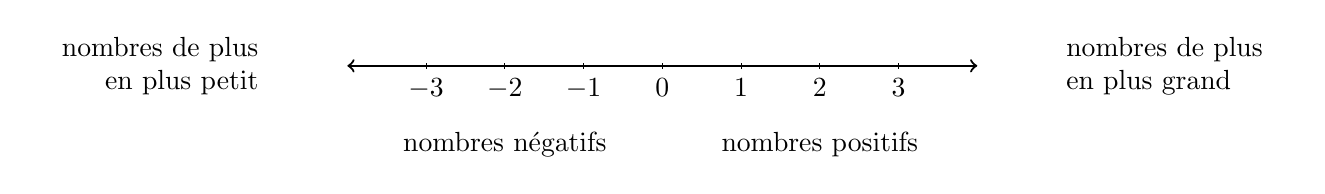
\begin{tikzpicture}
		\foreach \x in {-3,-2,-1,0,1,2,3}
   		\draw (\x cm,1pt) -- (\x cm,-1pt) node[anchor=north] {$\x$};

		\draw[thick,<->]
			node[anchor=east, align = right, text width = 80] at (-5,0) {nombres de plus en plus petit}
			node[anchor=center, align = right] at (-2,-1) {nombres négatifs}
			(-4,0) -- (4,0)
			node[anchor=center, align = left] at (2,-1) {nombres positifs}
			node[anchor=west, text width = 80] at (5,0) {nombres de plus en plus grand} ;
	\end{tikzpicture}
\end{center}

\noindent On introduit alors le concept de \emph{nombre négatif}, soit des nombres plus petit que 0. Pour avoir un nom commun à tous ces nombres, nous créons le concept de \emph{nombre relatif}, soit un nombre qui peut-être positif ou négatif. Les nombres négatifs ont un signe $-$ devant (par exemple, $-2$). Les \emph{nombres positifs}, soit ceux que nous connaissons déjà, ont soit un signe $+$ devant, soit aucun signe (par exemple, 3 ou $+9$).

\begin{exemple}
	Différentes écritures équivalentes (qui veulent dire la même chose):
	\begin{alignat*}{2}
		& \ 3 - 2\\
		= &\ 3 + (-2)\\
		= & +3 - 2\\
		= & +3 + (-2)\\
	\end{alignat*}
\end{exemple}
\noindent Nous introduisons aussi le concept d'\emph{opposé}.

\begin{definition}
	L'opposé d'un nombre est le nombre qui, ajouté à celui-ci, donne 0.
\end{definition}

\begin{exemple}
	$-3$ est l'opposé de 3 car $3 + (-3) = 3 -3 = 0$. 2 est l'opposé de $-2$ car $-2 + 2 = 2 + (-2) = 2 - 2 = 0$.
\end{exemple}

\noindent 0 est positif et négatif. Il est donc son propre opposé.

\begin{exercice}
	Quel est l'opposé de 12? De $-5$? De 0? De $8.5$? De $-181.9$?
\end{exercice}




\section{Règles de calcul}

\subsection{Règle des signes}

Que se passe-t-il quand deux signes se suivent? Les règles ci-dessous sont appliquées.

\begin{center}
	\begin{table}[h]
		\centering
		\begin{tabular}{|c|c|}
		\hline
		\textbf{Signes} & \textbf{Résultat} \\ \hline
		$+$ et $+$ & $+$ \\ \hline
		$-$ et $-$ & $+$ \\ \hline
		$+$ et $-$ & $-$ \\ \hline
		$-$ et $+$ & $-$ \\ \hline
		\end{tabular}
		\label{reglesdessignes}
		\end{table}
\end{center}

\vspace{-13mm}

\begin{exemple}
	$+ +3 = 3$, $- - 3 = 3$, $+-3 = -3$ et $-+3 = -3$.
\end{exemple}

\begin{astuce}
	Une bonne règle pour se souvenir de la règle des signe: l'ami de mon ami est mon ami, l'ennemi de mon ennemi est mon ennemi, l'ami de mon ennemi est mon ennemi et l'ennemi de mon ami est mon ennemi.
\end{astuce}

\begin{exercice}
	Simplifie les signes suivants: $+- 9$, $-- 10$, $-+ 0$.
\end{exercice}


\subsection{Reformulation de la soustraction}

\begin{propriete}
	Soustraire un nombre est équivalent à ajouter son opposé.
\end{propriete}

\begin{exemple}
	$19 - 8 = 19 + (-8) = 11$.
\end{exemple}

\begin{exercice}
	Calcule les résultats des opérations suivantes: $9-3$, $9+(-5)$, $5-9$, $0-1$, $-83-12$.
\end{exercice}



\subsection{Ordre}

\begin{propriete}
	Prenons deux nombres. S'ils sont de signe positif, ils respectent la règle de l'ordre que nous connaissons. Si les deux nombres sont de signe opposés, le plus petit est le négatif. S'ils sont tous les deux négatifs, ils sont rangés dans l'ordre inverse de leur opposés.
\end{propriete}

\begin{exemple}
	$2<5$, $-2< 1$, $6> -4$, $-2> -3$ et $-6< -1$.
\end{exemple}

\begin{exercice}
	Range dans l'ordre croissant les nombres suivants: 5, 9, $-1$, $-10$, $7.8$, 0, $-29.3$, $-29$, $-28$, $-29.6$.
\end{exercice}

\subsection{Produit}

\begin{propriete}
	Pour calculer le produit de deux nombres relatifs, on commence par calculer le résultat en ignorant les signes. Puis, on applique la règle des signes aux signes et on applique ce signe au résultat du produit.
\end{propriete}

\begin{exemple}
	Pour calculer $5 \times -3$, on fait $5 \times 3 = 15$. Puis, d'après la règle des signes, on a $+ - = -$. Donc le résultat est $-15$.
\end{exemple}

\begin{exercice}
	Effectue les calculs suivants: $-8 \times 2$, $-7 \times -7$, $0 \times -1$.
\end{exercice}